\chapter{Mechanik}

\renewcommand{\kapitelautor}{Autor: Alexander Punz}

\section{Rotorschutz}
In dem gewählten Bausatz des Hexacopters ist kein Rotorschutz beinhaltet, eines der Zeile ist es den Rotor möglichst gut zu schützen und das maximale Abfluggewicht nicht zu überschreiten. Da der Hexacopter mit einer maximalen Last von 1,9 kg belastet werden kann, können Materialen wie Stahl oder Aluminium für den Rotorschutz nicht verwendet werden. 
Da die Möglichkeit besteht, Teile in einer vernünftigen Qualität vor Ort drucken zu können, wurde die Fertigung mittels des 3D-Druckers gewählt. Mit diesem ist es möglich den erforderlichen Rotorschutz sehr genau und leicht drucken zu können. 
Die folgende Abbildung zeigt den fertigen Rotorschutz.

\begin{figure}[tbh]
\begin{centering}
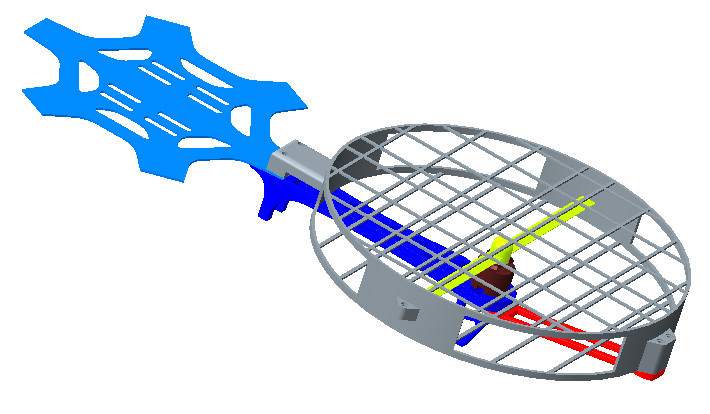
\includegraphics[width = 100mm]{Bilder/rotorschutz_zusammenbau}
\par\end{centering}
\caption{Rotorschutz systematisch dargestellt}
\label{Rotorschutz}
\end{figure}

Der Rotorschutz umrandet den Propeller, damit dieser im Falle eines Absturzes nicht zerstört wird. Die Lamellen ober- und unterhalb des Rotors sollen Personen gegen Verletzungen schützen. 
Der Ring wird durch die Strebe (rot) gestützt, damit er nicht nach unten abbrechen kann. 
Durch die großen Abmessungen bzw. der Form, kann der Ring nicht als ein Teil gedruckt werden, er wird dadurch in verschiedene Sektoren unterteilt. Der Ring wird in eine untere und obere Hälfte unterteilt bzw. beide Hälften wieder in zwei Teile. Die einzelnen Glieder werden dann mit Schrauben und Zweikomponentenkleber zusammengefügt. 

\section{Platinen}
Um das Projekt umsetzen zu können, ist es erforderlich einerseits den Mikroprozessor mit den Sensoren zu verbinden und andererseits die Kommunikation zwischen der Speisekarten-App und dem Hexacopter zu können. 
Damit diese Funktionen erfüllt werden können, werden zwei Platinen verwendet.

Das wichtigsten Bauteilgruppen der Kommunikationsplatine sind das WLAN-Modul, dieses ermöglicht die Kommunikation zwischen der App und dem Hexacopter und der Spannungsregler. Der Spannungsregler sorgt dafür, dass das WLAN-Modul mit 3.3 V versorgt wird und der Rest der Platine mit 5 V.
Die Hauptplatine beinhaltet ebenso mehrere Bereiche: Den Multiplexer, den Mikroprozessor und die Steckverbindungen für die einzelnen Sensoren.
Der Multiplexer wechslet zwischen der Steuerung der Flugmodi durch die Fernbedienung oder dem Mikroprozessor.

\begin{figure}[tbh]
\begin{centering}
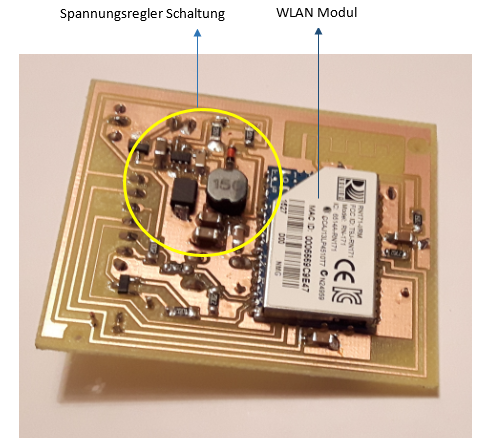
\includegraphics[width = 100mm]{Bilder/WP_Bottom_Beschriftung}
\par\end{centering}
\caption{Kommunikationsplatine Unterseite}
\label{WLAN Platine}
\end{figure}

\begin{figure}[tbh]
\begin{centering}
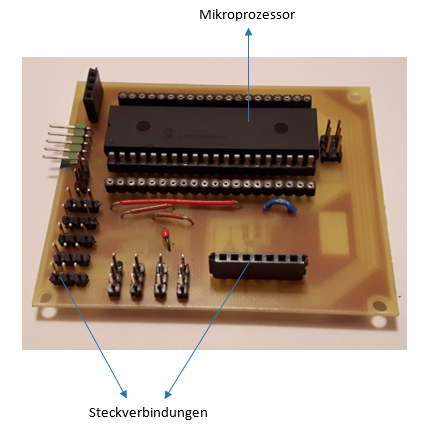
\includegraphics[width = 100mm]{Bilder/HP_Top_Beschriftung}
\par\end{centering}
\caption{Sensorplatine Oberseite}
\label{Sensor Platine oben}
\end{figure}


\begin{figure}[tbh]
\begin{centering}
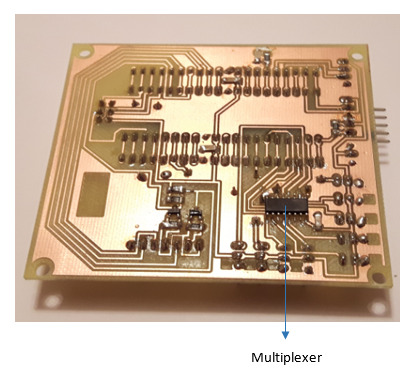
\includegraphics[width=100mm]{Bilder/HP_Bottom_Beschriftung}
\par\end{centering}
\caption{Sensorplatine Unterseite}
\label{Sensor Platine unten}
\end{figure}